\documentclass[1p]{elsarticle_modified}
%\bibliographystyle{elsarticle-num}

%\usepackage[colorlinks]{hyperref}
%\usepackage{abbrmath_seonhwa} %\Abb, \Ascr, \Acal ,\Abf, \Afrak
\usepackage{amsfonts}
\usepackage{amssymb}
\usepackage{amsmath}
\usepackage{amsthm}
\usepackage{scalefnt}
\usepackage{amsbsy}
\usepackage{kotex}
\usepackage{caption}
\usepackage{subfig}
\usepackage{color}
\usepackage{graphicx}
\usepackage{xcolor} %% white, black, red, green, blue, cyan, magenta, yellow
\usepackage{float}
\usepackage{setspace}
\usepackage{hyperref}

\usepackage{tikz}
\usetikzlibrary{arrows}

\usepackage{multirow}
\usepackage{array} % fixed length table
\usepackage{hhline}

%%%%%%%%%%%%%%%%%%%%%
\makeatletter
\renewcommand*\env@matrix[1][\arraystretch]{%
	\edef\arraystretch{#1}%
	\hskip -\arraycolsep
	\let\@ifnextchar\new@ifnextchar
	\array{*\c@MaxMatrixCols c}}
\makeatother %https://tex.stackexchange.com/questions/14071/how-can-i-increase-the-line-spacing-in-a-matrix
%%%%%%%%%%%%%%%

\usepackage[normalem]{ulem}

\newcommand{\msout}[1]{\ifmmode\text{\sout{\ensuremath{#1}}}\else\sout{#1}\fi}
%SOURCE: \msout is \stkout macro in https://tex.stackexchange.com/questions/20609/strikeout-in-math-mode

\newcommand{\cancel}[1]{
	\ifmmode
	{\color{red}\msout{#1}}
	\else
	{\color{red}\sout{#1}}
	\fi
}

\newcommand{\add}[1]{
	{\color{blue}\uwave{#1}}
}

\newcommand{\replace}[2]{
	\ifmmode
	{\color{red}\msout{#1}}{\color{blue}\uwave{#2}}
	\else
	{\color{red}\sout{#1}}{\color{blue}\uwave{#2}}
	\fi
}

\newcommand{\Sol}{\mathcal{S}} %segment
\newcommand{\D}{D} %diagram
\newcommand{\A}{\mathcal{A}} %arc


%%%%%%%%%%%%%%%%%%%%%%%%%%%%%5 test

\def\sl{\operatorname{\textup{SL}}(2,\Cbb)}
\def\psl{\operatorname{\textup{PSL}}(2,\Cbb)}
\def\quan{\mkern 1mu \triangleright \mkern 1mu}

\theoremstyle{definition}
\newtheorem{thm}{Theorem}[section]
\newtheorem{prop}[thm]{Proposition}
\newtheorem{lem}[thm]{Lemma}
\newtheorem{ques}[thm]{Question}
\newtheorem{cor}[thm]{Corollary}
\newtheorem{defn}[thm]{Definition}
\newtheorem{exam}[thm]{Example}
\newtheorem{rmk}[thm]{Remark}
\newtheorem{alg}[thm]{Algorithm}

\newcommand{\I}{\sqrt{-1}}
\begin{document}

%\begin{frontmatter}
%
%\title{Boundary parabolic representations of knots up to 8 crossings}
%
%%% Group authors per affiliation:
%\author{Yunhi Cho} 
%\address{Department of Mathematics, University of Seoul, Seoul, Korea}
%\ead{yhcho@uos.ac.kr}
%
%
%\author{Seonhwa Kim} %\fnref{s_kim}}
%\address{Center for Geometry and Physics, Institute for Basic Science, Pohang, 37673, Korea}
%\ead{ryeona17@ibs.re.kr}
%
%\author{Hyuk Kim}
%\address{Department of Mathematical Sciences, Seoul National University, Seoul 08826, Korea}
%\ead{hyukkim@snu.ac.kr}
%
%\author{Seokbeom Yoon}
%\address{Department of Mathematical Sciences, Seoul National University, Seoul, 08826,  Korea}
%\ead{sbyoon15@snu.ac.kr}
%
%\begin{abstract}
%We find all boundary parabolic representation of knots up to 8 crossings.
%
%\end{abstract}
%\begin{keyword}
%    \MSC[2010] 57M25 
%\end{keyword}
%
%\end{frontmatter}

%\linenumbers
%\tableofcontents
%
\newcommand\colored[1]{\textcolor{white}{\rule[-0.35ex]{0.8em}{1.4ex}}\kern-0.8em\color{red} #1}%
%\newcommand\colored[1]{\textcolor{white}{ #1}\kern-2.17ex	\textcolor{white}{ #1}\kern-1.81ex	\textcolor{white}{ #1}\kern-2.15ex\color{red}#1	}

{\Large $\underline{12n_{0731}~(K12n_{0731})}$}

\setlength{\tabcolsep}{10pt}
\renewcommand{\arraystretch}{1.6}
\vspace{1cm}\begin{tabular}{m{100pt}>{\centering\arraybackslash}m{274pt}}
\multirow{5}{120pt}{
	\centering
	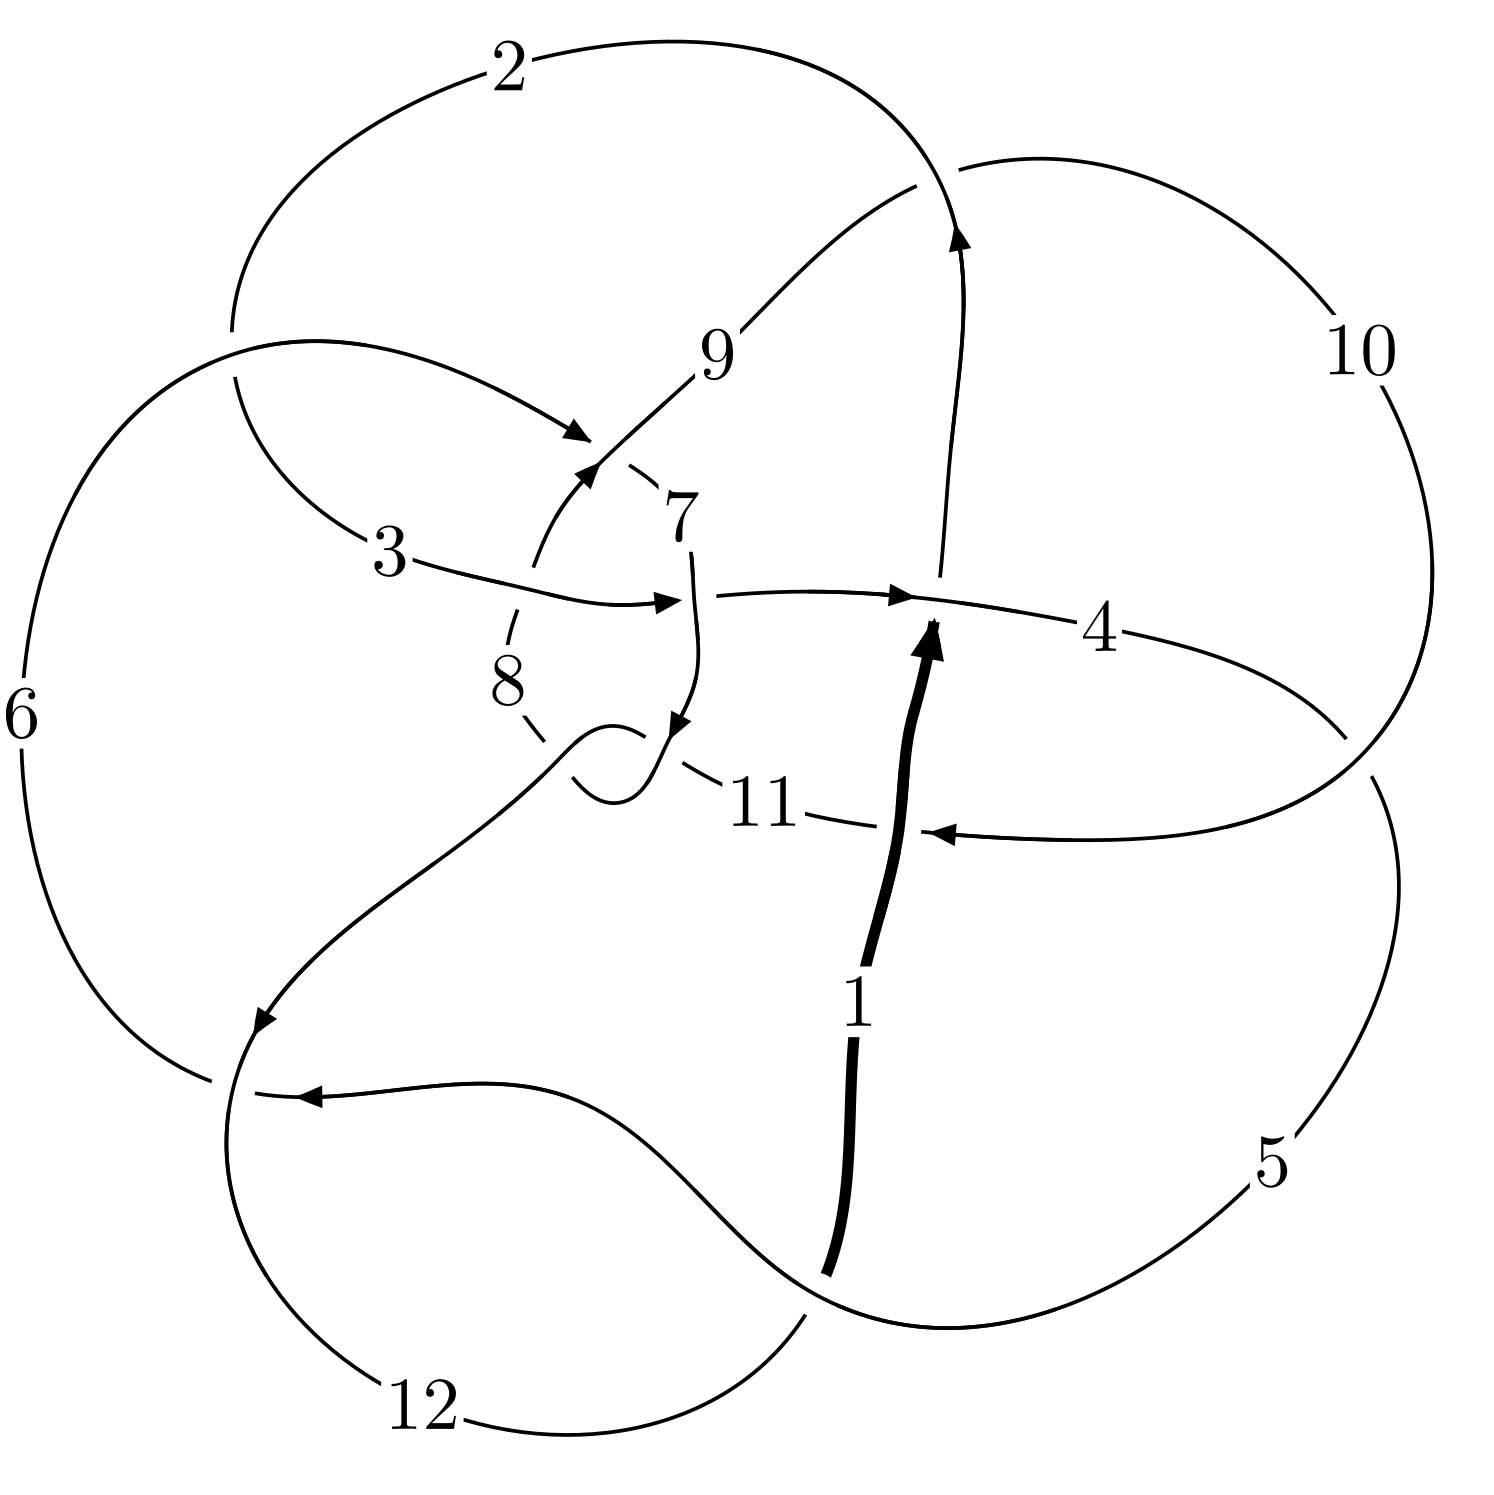
\includegraphics[width=112pt]{../../../GIT/diagram.site/Diagrams/png/2820_12n_0731.png}\\
\ \ \ A knot diagram\footnotemark}&
\allowdisplaybreaks
\textbf{Linearized knot diagam} \\
\cline{2-2}
 &
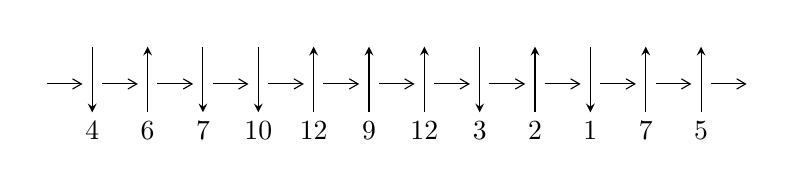
\begin{tikzpicture}[x=20pt, y=17pt]
	% nodes
	\node (C0) at (0, 0) {};
	\node (C1) at (1, 0) {};
	\node (C1U) at (1, +1) {};
	\node (C1D) at (1, -1) {4};

	\node (C2) at (2, 0) {};
	\node (C2U) at (2, +1) {};
	\node (C2D) at (2, -1) {6};

	\node (C3) at (3, 0) {};
	\node (C3U) at (3, +1) {};
	\node (C3D) at (3, -1) {7};

	\node (C4) at (4, 0) {};
	\node (C4U) at (4, +1) {};
	\node (C4D) at (4, -1) {10};

	\node (C5) at (5, 0) {};
	\node (C5U) at (5, +1) {};
	\node (C5D) at (5, -1) {12};

	\node (C6) at (6, 0) {};
	\node (C6U) at (6, +1) {};
	\node (C6D) at (6, -1) {9};

	\node (C7) at (7, 0) {};
	\node (C7U) at (7, +1) {};
	\node (C7D) at (7, -1) {12};

	\node (C8) at (8, 0) {};
	\node (C8U) at (8, +1) {};
	\node (C8D) at (8, -1) {3};

	\node (C9) at (9, 0) {};
	\node (C9U) at (9, +1) {};
	\node (C9D) at (9, -1) {2};

	\node (C10) at (10, 0) {};
	\node (C10U) at (10, +1) {};
	\node (C10D) at (10, -1) {1};

	\node (C11) at (11, 0) {};
	\node (C11U) at (11, +1) {};
	\node (C11D) at (11, -1) {7};

	\node (C12) at (12, 0) {};
	\node (C12U) at (12, +1) {};
	\node (C12D) at (12, -1) {5};
	\node (C13) at (13, 0) {};

	% arrows
	\draw[->,>={angle 60}]
	(C0) edge (C1) (C1) edge (C2) (C2) edge (C3) (C3) edge (C4) (C4) edge (C5) (C5) edge (C6) (C6) edge (C7) (C7) edge (C8) (C8) edge (C9) (C9) edge (C10) (C10) edge (C11) (C11) edge (C12) (C12) edge (C13) ;	\draw[->,>=stealth]
	(C1U) edge (C1D) (C2D) edge (C2U) (C3U) edge (C3D) (C4U) edge (C4D) (C5D) edge (C5U) (C6D) edge (C6U) (C7D) edge (C7U) (C8U) edge (C8D) (C9D) edge (C9U) (C10U) edge (C10D) (C11D) edge (C11U) (C12D) edge (C12U) ;
	\end{tikzpicture} \\
\hhline{~~} \\& 
\textbf{Solving Sequence} \\ \cline{2-2} 
 &
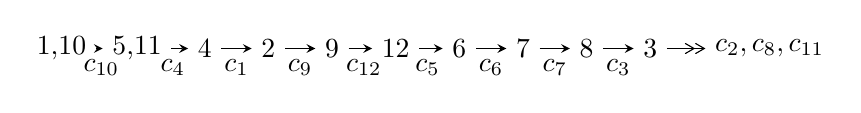
\begin{tikzpicture}[x=23pt, y=7pt]
	% node
	\node (A0) at (-1/8, 0) {1,10};
	\node (A1) at (17/16, 0) {5,11};
	\node (A2) at (17/8, 0) {4};
	\node (A3) at (25/8, 0) {2};
	\node (A4) at (33/8, 0) {9};
	\node (A5) at (41/8, 0) {12};
	\node (A6) at (49/8, 0) {6};
	\node (A7) at (57/8, 0) {7};
	\node (A8) at (65/8, 0) {8};
	\node (A9) at (73/8, 0) {3};
	\node (C1) at (1/2, -1) {$c_{10}$};
	\node (C2) at (13/8, -1) {$c_{4}$};
	\node (C3) at (21/8, -1) {$c_{1}$};
	\node (C4) at (29/8, -1) {$c_{9}$};
	\node (C5) at (37/8, -1) {$c_{12}$};
	\node (C6) at (45/8, -1) {$c_{5}$};
	\node (C7) at (53/8, -1) {$c_{6}$};
	\node (C8) at (61/8, -1) {$c_{7}$};
	\node (C9) at (69/8, -1) {$c_{3}$};
	\node (A10) at (11, 0) {$c_{2},c_{8},c_{11}$};

	% edge
	\draw[->,>=stealth]	
	(A0) edge (A1) (A1) edge (A2) (A2) edge (A3) (A3) edge (A4) (A4) edge (A5) (A5) edge (A6) (A6) edge (A7) (A7) edge (A8) (A8) edge (A9) ;
	\draw[->>,>={angle 60}]	
	(A9) edge (A10);
\end{tikzpicture} \\ 

\end{tabular} \\

\footnotetext{
The image of knot diagram is generated by the software ``\textbf{Draw programme}" developed by Andrew Bartholomew(\url{http://www.layer8.co.uk/maths/draw/index.htm\#Running-draw}), where we modified some parts for our purpose(\url{https://github.com/CATsTAILs/LinksPainter}).
}\phantom \\ \newline 
\centering \textbf{Ideals for irreducible components\footnotemark of $X_{\text{par}}$} 
 
\begin{align*}
I^u_{1}&=\langle 
3.93575\times10^{718} u^{105}+3.48971\times10^{719} u^{104}+\cdots+3.15936\times10^{722} b+1.38793\times10^{723},\\
\phantom{I^u_{1}}&\phantom{= \langle  }-5.52453\times10^{723} u^{105}-5.11171\times10^{724} u^{104}+\cdots+9.52365\times10^{725} a-1.77941\times10^{728},\\
\phantom{I^u_{1}}&\phantom{= \langle  }u^{106}+10 u^{105}+\cdots-15333 u+21101\rangle \\
I^u_{2}&=\langle 
4.63757\times10^{102} u^{45}-4.96173\times10^{103} u^{44}+\cdots+2.96832\times10^{102} b-1.06364\times10^{103},\\
\phantom{I^u_{2}}&\phantom{= \langle  }-4.46704\times10^{101} u^{45}+4.84639\times10^{102} u^{44}+\cdots+1.09938\times10^{101} a+4.31174\times10^{101},\\
\phantom{I^u_{2}}&\phantom{= \langle  }u^{46}-11 u^{45}+\cdots-7 u+1\rangle \\
\\
\end{align*}
\raggedright * 2 irreducible components of $\dim_{\mathbb{C}}=0$, with total 152 representations.\\
\footnotetext{All coefficients of polynomials are rational numbers. But the coefficients are sometimes approximated in decimal forms when there is not enough margin.}
\newpage
\renewcommand{\arraystretch}{1}
\centering \section*{I. $I^u_{1}= \langle 3.94\times10^{718} u^{105}+3.49\times10^{719} u^{104}+\cdots+3.16\times10^{722} b+1.39\times10^{723},\;-5.52\times10^{723} u^{105}-5.11\times10^{724} u^{104}+\cdots+9.52\times10^{725} a-1.78\times10^{728},\;u^{106}+10 u^{105}+\cdots-15333 u+21101 \rangle$}
\flushleft \textbf{(i) Arc colorings}\\
\begin{tabular}{m{7pt} m{180pt} m{7pt} m{180pt} }
\flushright $a_{1}=$&$\begin{pmatrix}0\\u\end{pmatrix}$ \\
\flushright $a_{10}=$&$\begin{pmatrix}1\\0\end{pmatrix}$ \\
\flushright $a_{5}=$&$\begin{pmatrix}0.00580085 u^{105}+0.0536738 u^{104}+\cdots-572.698 u+186.841\\-0.000124574 u^{105}-0.00110456 u^{104}+\cdots+24.9971 u-4.39308\end{pmatrix}$ \\
\flushright $a_{11}=$&$\begin{pmatrix}1\\u^2\end{pmatrix}$ \\
\flushright $a_{4}=$&$\begin{pmatrix}0.00567627 u^{105}+0.0525692 u^{104}+\cdots-547.701 u+182.448\\-0.000124574 u^{105}-0.00110456 u^{104}+\cdots+24.9971 u-4.39308\end{pmatrix}$ \\
\flushright $a_{2}=$&$\begin{pmatrix}-0.000537252 u^{105}-0.000473389 u^{104}+\cdots-629.847 u+113.927\\-0.00320183 u^{105}-0.0290170 u^{104}+\cdots+170.414 u-77.5333\end{pmatrix}$ \\
\flushright $a_{9}=$&$\begin{pmatrix}0.00921004 u^{105}+0.0926336 u^{104}+\cdots-2089.53 u+697.826\\-0.00291743 u^{105}-0.0260276 u^{104}+\cdots+39.1070 u-48.6936\end{pmatrix}$ \\
\flushright $a_{12}=$&$\begin{pmatrix}0.00598408 u^{105}+0.0586924 u^{104}+\cdots-978.692 u+272.862\\-0.00331950 u^{105}-0.0301488 u^{104}+\cdots+180.431 u-81.4016\end{pmatrix}$ \\
\flushright $a_{6}=$&$\begin{pmatrix}-0.0526098 u^{105}-0.500361 u^{104}+\cdots+5932.15 u-2233.30\\-0.000768914 u^{105}-0.00825865 u^{104}+\cdots+242.812 u-76.3708\end{pmatrix}$ \\
\flushright $a_{7}=$&$\begin{pmatrix}0.000439883 u^{105}+0.000487826 u^{104}+\cdots+1000.19 u-186.949\\0.000546921 u^{105}+0.00460690 u^{104}+\cdots+40.0615 u-4.47173\end{pmatrix}$ \\
\flushright $a_{8}=$&$\begin{pmatrix}-0.0234483 u^{105}-0.233104 u^{104}+\cdots+4664.71 u-1533.64\\-0.00343512 u^{105}-0.0330149 u^{104}+\cdots+409.086 u-149.387\end{pmatrix}$ \\
\flushright $a_{3}=$&$\begin{pmatrix}0.0268396 u^{105}+0.252050 u^{104}+\cdots-3022.06 u+1070.17\\0.00293758 u^{105}+0.0273639 u^{104}+\cdots-238.020 u+100.084\end{pmatrix}$\\&\end{tabular}
\flushleft \textbf{(ii) Obstruction class $= -1$}\\~\\
\flushleft \textbf{(iii) Cusp Shapes $= 0.0420363 u^{105}+0.394092 u^{104}+\cdots-4107.71 u+1589.71$}\\~\\
\newpage\renewcommand{\arraystretch}{1}
\flushleft \textbf{(iv) u-Polynomials at the component}\newline \\
\begin{tabular}{m{50pt}|m{274pt}}
Crossings & \hspace{64pt}u-Polynomials at each crossing \\
\hline $$\begin{aligned}c_{1}\end{aligned}$$&$\begin{aligned}
&u^{106}+4 u^{105}+\cdots+166 u+7
\end{aligned}$\\
\hline $$\begin{aligned}c_{2}\end{aligned}$$&$\begin{aligned}
&u^{106}-2 u^{105}+\cdots-689301 u+133281
\end{aligned}$\\
\hline $$\begin{aligned}c_{3}\end{aligned}$$&$\begin{aligned}
&u^{106}+3 u^{105}+\cdots-4214426643 u+4151404117
\end{aligned}$\\
\hline $$\begin{aligned}c_{4}\end{aligned}$$&$\begin{aligned}
&u^{106}-2 u^{105}+\cdots-717 u+99
\end{aligned}$\\
\hline $$\begin{aligned}c_{5},c_{12}\end{aligned}$$&$\begin{aligned}
&u^{106}-2 u^{105}+\cdots+1381696 u+76939
\end{aligned}$\\
\hline $$\begin{aligned}c_{6}\end{aligned}$$&$\begin{aligned}
&u^{106}+7 u^{105}+\cdots+4 u+1
\end{aligned}$\\
\hline $$\begin{aligned}c_{7},c_{11}\end{aligned}$$&$\begin{aligned}
&u^{106}-2 u^{105}+\cdots+2088059 u+2311849
\end{aligned}$\\
\hline $$\begin{aligned}c_{8}\end{aligned}$$&$\begin{aligned}
&u^{106}+u^{105}+\cdots-233910687 u+50664949
\end{aligned}$\\
\hline $$\begin{aligned}c_{9}\end{aligned}$$&$\begin{aligned}
&u^{106}-2 u^{105}+\cdots+701049191 u+114592757
\end{aligned}$\\
\hline $$\begin{aligned}c_{10}\end{aligned}$$&$\begin{aligned}
&u^{106}-10 u^{105}+\cdots+15333 u+21101
\end{aligned}$\\
\hline
\end{tabular}\\~\\
\newpage\renewcommand{\arraystretch}{1}
\flushleft \textbf{(v) Riley Polynomials at the component}\newline \\
\begin{tabular}{m{50pt}|m{274pt}}
Crossings & \hspace{64pt}Riley Polynomials at each crossing \\
\hline $$\begin{aligned}c_{1}\end{aligned}$$&$\begin{aligned}
&y^{106}-20 y^{105}+\cdots+1704 y+49
\end{aligned}$\\
\hline $$\begin{aligned}c_{2}\end{aligned}$$&$\begin{aligned}
&y^{106}+46 y^{105}+\cdots+3044616486147 y+17763824961
\end{aligned}$\\
\hline $$\begin{aligned}c_{3}\end{aligned}$$&$\begin{aligned}
&y^{106}-59 y^{105}+\cdots-3.51\times10^{20} y+1.72\times10^{19}
\end{aligned}$\\
\hline $$\begin{aligned}c_{4}\end{aligned}$$&$\begin{aligned}
&y^{106}-8 y^{105}+\cdots-558243 y+9801
\end{aligned}$\\
\hline $$\begin{aligned}c_{5},c_{12}\end{aligned}$$&$\begin{aligned}
&y^{106}+116 y^{105}+\cdots+9155464634 y+5919609721
\end{aligned}$\\
\hline $$\begin{aligned}c_{6}\end{aligned}$$&$\begin{aligned}
&y^{106}-7 y^{105}+\cdots+382 y+1
\end{aligned}$\\
\hline $$\begin{aligned}c_{7},c_{11}\end{aligned}$$&$\begin{aligned}
&y^{106}+100 y^{105}+\cdots+37507627368405 y+5344645798801
\end{aligned}$\\
\hline $$\begin{aligned}c_{8}\end{aligned}$$&$\begin{aligned}
&y^{106}-51 y^{105}+\cdots-49138395059999669 y+2566937057172601
\end{aligned}$\\
\hline $$\begin{aligned}c_{9}\end{aligned}$$&$\begin{aligned}
&y^{106}+64 y^{105}+\cdots+722400296247735653 y+13131499956861049
\end{aligned}$\\
\hline $$\begin{aligned}c_{10}\end{aligned}$$&$\begin{aligned}
&y^{106}-48 y^{105}+\cdots+110688846921 y+445252201
\end{aligned}$\\
\hline
\end{tabular}\\~\\
\newpage\flushleft \textbf{(vi) Complex Volumes and Cusp Shapes}
$$\begin{array}{c|c|c}  
\text{Solutions to }I^u_{1}& \I (\text{vol} + \sqrt{-1}CS) & \text{Cusp shape}\\
 \hline 
\begin{aligned}
u &= \phantom{-}0.948251 + 0.358375 I \\
a &= -0.154934 - 0.911130 I \\
b &= -0.510751 + 1.304030 I\end{aligned}
 & -0.767957 + 0.562214 I & \phantom{-0.000000 } 0 \\ \hline\begin{aligned}
u &= \phantom{-}0.948251 - 0.358375 I \\
a &= -0.154934 + 0.911130 I \\
b &= -0.510751 - 1.304030 I\end{aligned}
 & -0.767957 - 0.562214 I & \phantom{-0.000000 } 0 \\ \hline\begin{aligned}
u &= -0.930685 + 0.254156 I \\
a &= \phantom{-}0.01050 + 1.63189 I \\
b &= -1.07268 - 1.48298 I\end{aligned}
 & -11.7927 + 9.8137 I & \phantom{-0.000000 } 0 \\ \hline\begin{aligned}
u &= -0.930685 - 0.254156 I \\
a &= \phantom{-}0.01050 - 1.63189 I \\
b &= -1.07268 + 1.48298 I\end{aligned}
 & -11.7927 - 9.8137 I & \phantom{-0.000000 } 0 \\ \hline\begin{aligned}
u &= -0.945138 + 0.053638 I \\
a &= -0.85171 + 1.91195 I \\
b &= -0.846585 - 0.188696 I\end{aligned}
 & -11.8754 - 8.4290 I & \phantom{-0.000000 } 0 \\ \hline\begin{aligned}
u &= -0.945138 - 0.053638 I \\
a &= -0.85171 - 1.91195 I \\
b &= -0.846585 + 0.188696 I\end{aligned}
 & -11.8754 + 8.4290 I & \phantom{-0.000000 } 0 \\ \hline\begin{aligned}
u &= -1.062100 + 0.135212 I \\
a &= \phantom{-}0.326050 + 0.030341 I \\
b &= -0.260804 - 0.164981 I\end{aligned}
 & \phantom{-}2.19964 - 0.01235 I & \phantom{-0.000000 } 0 \\ \hline\begin{aligned}
u &= -1.062100 - 0.135212 I \\
a &= \phantom{-}0.326050 - 0.030341 I \\
b &= -0.260804 + 0.164981 I\end{aligned}
 & \phantom{-}2.19964 + 0.01235 I & \phantom{-0.000000 } 0 \\ \hline\begin{aligned}
u &= -0.782358 + 0.742448 I \\
a &= \phantom{-}0.92375 - 1.12045 I \\
b &= -0.776614 + 0.856855 I\end{aligned}
 & -6.70297 + 3.11731 I & \phantom{-0.000000 } 0 \\ \hline\begin{aligned}
u &= -0.782358 - 0.742448 I \\
a &= \phantom{-}0.92375 + 1.12045 I \\
b &= -0.776614 - 0.856855 I\end{aligned}
 & -6.70297 - 3.11731 I & \phantom{-0.000000 } 0\\
 \hline 
 \end{array}$$\newpage$$\begin{array}{c|c|c}  
\text{Solutions to }I^u_{1}& \I (\text{vol} + \sqrt{-1}CS) & \text{Cusp shape}\\
 \hline 
\begin{aligned}
u &= -1.095120 + 0.119769 I \\
a &= \phantom{-}0.264555 + 1.382680 I \\
b &= -1.10117 - 1.34433 I\end{aligned}
 & -11.66480 + 1.74888 I & \phantom{-0.000000 } 0 \\ \hline\begin{aligned}
u &= -1.095120 - 0.119769 I \\
a &= \phantom{-}0.264555 - 1.382680 I \\
b &= -1.10117 + 1.34433 I\end{aligned}
 & -11.66480 - 1.74888 I & \phantom{-0.000000 } 0 \\ \hline\begin{aligned}
u &= \phantom{-}0.797748 + 0.760470 I \\
a &= \phantom{-}1.08756 - 1.39027 I \\
b &= \phantom{-}0.693867 + 0.683785 I\end{aligned}
 & -6.23465 - 1.54870 I & \phantom{-0.000000 } 0 \\ \hline\begin{aligned}
u &= \phantom{-}0.797748 - 0.760470 I \\
a &= \phantom{-}1.08756 + 1.39027 I \\
b &= \phantom{-}0.693867 - 0.683785 I\end{aligned}
 & -6.23465 + 1.54870 I & \phantom{-0.000000 } 0 \\ \hline\begin{aligned}
u &= -0.850488 + 0.260836 I \\
a &= \phantom{-}0.70300 - 1.65375 I \\
b &= \phantom{-}1.134180 + 0.421351 I\end{aligned}
 & -10.10390 + 2.94022 I & \phantom{-0.000000 } 0 \\ \hline\begin{aligned}
u &= -0.850488 - 0.260836 I \\
a &= \phantom{-}0.70300 + 1.65375 I \\
b &= \phantom{-}1.134180 - 0.421351 I\end{aligned}
 & -10.10390 - 2.94022 I & \phantom{-0.000000 } 0 \\ \hline\begin{aligned}
u &= -0.942406 + 0.605035 I \\
a &= -0.73783 + 1.25298 I \\
b &= \phantom{-}1.57100 - 1.20619 I\end{aligned}
 & -7.51559 + 5.45810 I & \phantom{-0.000000 } 0 \\ \hline\begin{aligned}
u &= -0.942406 - 0.605035 I \\
a &= -0.73783 - 1.25298 I \\
b &= \phantom{-}1.57100 + 1.20619 I\end{aligned}
 & -7.51559 - 5.45810 I & \phantom{-0.000000 } 0 \\ \hline\begin{aligned}
u &= -0.793473 + 0.794434 I \\
a &= -0.22967 - 1.45133 I \\
b &= -0.784680 + 0.922555 I\end{aligned}
 & \phantom{-}3.59008 + 5.00840 I & \phantom{-0.000000 } 0 \\ \hline\begin{aligned}
u &= -0.793473 - 0.794434 I \\
a &= -0.22967 + 1.45133 I \\
b &= -0.784680 - 0.922555 I\end{aligned}
 & \phantom{-}3.59008 - 5.00840 I & \phantom{-0.000000 } 0\\
 \hline 
 \end{array}$$\newpage$$\begin{array}{c|c|c}  
\text{Solutions to }I^u_{1}& \I (\text{vol} + \sqrt{-1}CS) & \text{Cusp shape}\\
 \hline 
\begin{aligned}
u &= -1.136930 + 0.025652 I \\
a &= \phantom{-}0.10186 + 1.44244 I \\
b &= \phantom{-}1.19216 - 1.13971 I\end{aligned}
 & -11.47160 + 1.76278 I & \phantom{-0.000000 } 0 \\ \hline\begin{aligned}
u &= -1.136930 - 0.025652 I \\
a &= \phantom{-}0.10186 - 1.44244 I \\
b &= \phantom{-}1.19216 + 1.13971 I\end{aligned}
 & -11.47160 - 1.76278 I & \phantom{-0.000000 } 0 \\ \hline\begin{aligned}
u &= -1.133530 + 0.262789 I \\
a &= \phantom{-}0.168383 - 0.318272 I \\
b &= -0.723006 + 0.657240 I\end{aligned}
 & \phantom{-}2.39981 + 0.29529 I & \phantom{-0.000000 } 0 \\ \hline\begin{aligned}
u &= -1.133530 - 0.262789 I \\
a &= \phantom{-}0.168383 + 0.318272 I \\
b &= -0.723006 - 0.657240 I\end{aligned}
 & \phantom{-}2.39981 - 0.29529 I & \phantom{-0.000000 } 0 \\ \hline\begin{aligned}
u &= -1.142390 + 0.245124 I \\
a &= -0.089472 - 0.364832 I \\
b &= -0.827228 + 0.837561 I\end{aligned}
 & \phantom{-}0.57325 + 8.04216 I & \phantom{-0.000000 } 0 \\ \hline\begin{aligned}
u &= -1.142390 - 0.245124 I \\
a &= -0.089472 + 0.364832 I \\
b &= -0.827228 - 0.837561 I\end{aligned}
 & \phantom{-}0.57325 - 8.04216 I & \phantom{-0.000000 } 0 \\ \hline\begin{aligned}
u &= -0.785176 + 0.240971 I \\
a &= \phantom{-}0.87091 - 1.86486 I \\
b &= \phantom{-}0.355226 + 0.832415 I\end{aligned}
 & -7.36655 + 1.24942 I & \phantom{-0.000000 } 0 \\ \hline\begin{aligned}
u &= -0.785176 - 0.240971 I \\
a &= \phantom{-}0.87091 + 1.86486 I \\
b &= \phantom{-}0.355226 - 0.832415 I\end{aligned}
 & -7.36655 - 1.24942 I & \phantom{-0.000000 } 0 \\ \hline\begin{aligned}
u &= \phantom{-}1.007270 + 0.634188 I \\
a &= -0.493189 + 0.266012 I \\
b &= -0.655674 + 0.146501 I\end{aligned}
 & -4.52914 - 1.62674 I & \phantom{-0.000000 } 0 \\ \hline\begin{aligned}
u &= \phantom{-}1.007270 - 0.634188 I \\
a &= -0.493189 - 0.266012 I \\
b &= -0.655674 - 0.146501 I\end{aligned}
 & -4.52914 + 1.62674 I & \phantom{-0.000000 } 0\\
 \hline 
 \end{array}$$\newpage$$\begin{array}{c|c|c}  
\text{Solutions to }I^u_{1}& \I (\text{vol} + \sqrt{-1}CS) & \text{Cusp shape}\\
 \hline 
\begin{aligned}
u &= -1.194200 + 0.015303 I \\
a &= \phantom{-}0.191122 - 1.267150 I \\
b &= \phantom{-}0.757365 + 0.167163 I\end{aligned}
 & -9.51831 + 1.58191 I & \phantom{-0.000000 } 0 \\ \hline\begin{aligned}
u &= -1.194200 - 0.015303 I \\
a &= \phantom{-}0.191122 + 1.267150 I \\
b &= \phantom{-}0.757365 - 0.167163 I\end{aligned}
 & -9.51831 - 1.58191 I & \phantom{-0.000000 } 0 \\ \hline\begin{aligned}
u &= \phantom{-}0.715283 + 0.362122 I \\
a &= \phantom{-}0.258748 + 0.444327 I \\
b &= -1.21522 - 0.89354 I\end{aligned}
 & \phantom{-}0.26251 - 5.29920 I & \phantom{-0.000000 } 0 \\ \hline\begin{aligned}
u &= \phantom{-}0.715283 - 0.362122 I \\
a &= \phantom{-}0.258748 - 0.444327 I \\
b &= -1.21522 + 0.89354 I\end{aligned}
 & \phantom{-}0.26251 + 5.29920 I & \phantom{-0.000000 } 0 \\ \hline\begin{aligned}
u &= \phantom{-}0.039556 + 0.776971 I \\
a &= -0.951114 - 0.865301 I \\
b &= -0.366670 + 1.048150 I\end{aligned}
 & \phantom{-}1.09346 - 2.32406 I & \phantom{-0.000000 } 0 \\ \hline\begin{aligned}
u &= \phantom{-}0.039556 - 0.776971 I \\
a &= -0.951114 + 0.865301 I \\
b &= -0.366670 - 1.048150 I\end{aligned}
 & \phantom{-}1.09346 + 2.32406 I & \phantom{-0.000000 } 0 \\ \hline\begin{aligned}
u &= \phantom{-}1.126670 + 0.522022 I \\
a &= -0.431260 - 1.241580 I \\
b &= \phantom{-}1.37061 + 1.09434 I\end{aligned}
 & -7.07297 - 0.53927 I & \phantom{-0.000000 } 0 \\ \hline\begin{aligned}
u &= \phantom{-}1.126670 - 0.522022 I \\
a &= -0.431260 + 1.241580 I \\
b &= \phantom{-}1.37061 - 1.09434 I\end{aligned}
 & -7.07297 + 0.53927 I & \phantom{-0.000000 } 0 \\ \hline\begin{aligned}
u &= \phantom{-}1.055460 + 0.681232 I \\
a &= \phantom{-}0.306393 + 0.858063 I \\
b &= -0.652118 + 0.095378 I\end{aligned}
 & -4.17577 + 1.05529 I & \phantom{-0.000000 } 0 \\ \hline\begin{aligned}
u &= \phantom{-}1.055460 - 0.681232 I \\
a &= \phantom{-}0.306393 - 0.858063 I \\
b &= -0.652118 - 0.095378 I\end{aligned}
 & -4.17577 - 1.05529 I & \phantom{-0.000000 } 0\\
 \hline 
 \end{array}$$\newpage$$\begin{array}{c|c|c}  
\text{Solutions to }I^u_{1}& \I (\text{vol} + \sqrt{-1}CS) & \text{Cusp shape}\\
 \hline 
\begin{aligned}
u &= \phantom{-}0.716244 + 1.049390 I \\
a &= -0.307272 - 0.800764 I \\
b &= \phantom{-}0.834602 + 0.837103 I\end{aligned}
 & \phantom{-}0.62607 - 2.48643 I & \phantom{-0.000000 } 0 \\ \hline\begin{aligned}
u &= \phantom{-}0.716244 - 1.049390 I \\
a &= -0.307272 + 0.800764 I \\
b &= \phantom{-}0.834602 - 0.837103 I\end{aligned}
 & \phantom{-}0.62607 + 2.48643 I & \phantom{-0.000000 } 0 \\ \hline\begin{aligned}
u &= \phantom{-}0.649056 + 1.129630 I \\
a &= -0.852304 - 0.606312 I \\
b &= \phantom{-}0.953022 + 0.164976 I\end{aligned}
 & -4.69259 - 5.04246 I & \phantom{-0.000000 } 0 \\ \hline\begin{aligned}
u &= \phantom{-}0.649056 - 1.129630 I \\
a &= -0.852304 + 0.606312 I \\
b &= \phantom{-}0.953022 - 0.164976 I\end{aligned}
 & -4.69259 + 5.04246 I & \phantom{-0.000000 } 0 \\ \hline\begin{aligned}
u &= \phantom{-}0.501347 + 0.472370 I \\
a &= -0.00844 + 1.77091 I \\
b &= -0.86573 - 1.27101 I\end{aligned}
 & \phantom{-}2.10442 - 3.12705 I & \phantom{-0.000000 } 0 \\ \hline\begin{aligned}
u &= \phantom{-}0.501347 - 0.472370 I \\
a &= -0.00844 - 1.77091 I \\
b &= -0.86573 + 1.27101 I\end{aligned}
 & \phantom{-}2.10442 + 3.12705 I & \phantom{-0.000000 } 0 \\ \hline\begin{aligned}
u &= -0.206688 + 0.653964 I \\
a &= -0.698029 - 0.144455 I \\
b &= \phantom{-}0.142044 + 1.053890 I\end{aligned}
 & \phantom{-}0.66152 - 1.95991 I & \phantom{-0.000000 } 0 \\ \hline\begin{aligned}
u &= -0.206688 - 0.653964 I \\
a &= -0.698029 + 0.144455 I \\
b &= \phantom{-}0.142044 - 1.053890 I\end{aligned}
 & \phantom{-}0.66152 + 1.95991 I & \phantom{-0.000000 } 0 \\ \hline\begin{aligned}
u &= -0.343078 + 0.550704 I \\
a &= \phantom{-}1.047830 + 0.746559 I \\
b &= \phantom{-}0.932482 - 0.842902 I\end{aligned}
 & \phantom{-}0.30226 + 3.78367 I & \phantom{-0.000000 } 0 \\ \hline\begin{aligned}
u &= -0.343078 - 0.550704 I \\
a &= \phantom{-}1.047830 - 0.746559 I \\
b &= \phantom{-}0.932482 + 0.842902 I\end{aligned}
 & \phantom{-}0.30226 - 3.78367 I & \phantom{-0.000000 } 0\\
 \hline 
 \end{array}$$\newpage$$\begin{array}{c|c|c}  
\text{Solutions to }I^u_{1}& \I (\text{vol} + \sqrt{-1}CS) & \text{Cusp shape}\\
 \hline 
\begin{aligned}
u &= -0.597051 + 0.247246 I \\
a &= \phantom{-}1.009150 + 0.086880 I \\
b &= \phantom{-}0.821278 - 0.470853 I\end{aligned}
 & -1.68666 + 1.98824 I & \phantom{-0.000000 } 0 \\ \hline\begin{aligned}
u &= -0.597051 - 0.247246 I \\
a &= \phantom{-}1.009150 - 0.086880 I \\
b &= \phantom{-}0.821278 + 0.470853 I\end{aligned}
 & -1.68666 - 1.98824 I & \phantom{-0.000000 } 0 \\ \hline\begin{aligned}
u &= \phantom{-}0.617618 + 0.183682 I \\
a &= \phantom{-}1.036030 + 0.858345 I \\
b &= \phantom{-}0.234908 + 0.223337 I\end{aligned}
 & \phantom{-}0.96810 + 1.47192 I & \phantom{-0.000000 } 0 \\ \hline\begin{aligned}
u &= \phantom{-}0.617618 - 0.183682 I \\
a &= \phantom{-}1.036030 - 0.858345 I \\
b &= \phantom{-}0.234908 - 0.223337 I\end{aligned}
 & \phantom{-}0.96810 - 1.47192 I & \phantom{-0.000000 } 0 \\ \hline\begin{aligned}
u &= \phantom{-}0.937954 + 1.003510 I \\
a &= \phantom{-}0.507532 - 1.161270 I \\
b &= \phantom{-}0.877508 + 0.856765 I\end{aligned}
 & -6.00148 - 10.91030 I & \phantom{-0.000000 } 0 \\ \hline\begin{aligned}
u &= \phantom{-}0.937954 - 1.003510 I \\
a &= \phantom{-}0.507532 + 1.161270 I \\
b &= \phantom{-}0.877508 - 0.856765 I\end{aligned}
 & -6.00148 + 10.91030 I & \phantom{-0.000000 } 0 \\ \hline\begin{aligned}
u &= \phantom{-}1.261480 + 0.596350 I \\
a &= \phantom{-}0.130770 + 0.811658 I \\
b &= -0.886100 - 0.141133 I\end{aligned}
 & -5.30219 - 1.09707 I & \phantom{-0.000000 } 0 \\ \hline\begin{aligned}
u &= \phantom{-}1.261480 - 0.596350 I \\
a &= \phantom{-}0.130770 - 0.811658 I \\
b &= -0.886100 + 0.141133 I\end{aligned}
 & -5.30219 + 1.09707 I & \phantom{-0.000000 } 0 \\ \hline\begin{aligned}
u &= \phantom{-}1.036710 + 0.951321 I \\
a &= -0.452856 + 0.505281 I \\
b &= \phantom{-}1.020630 - 0.738227 I\end{aligned}
 & -6.47476 - 4.69639 I & \phantom{-0.000000 } 0 \\ \hline\begin{aligned}
u &= \phantom{-}1.036710 - 0.951321 I \\
a &= -0.452856 - 0.505281 I \\
b &= \phantom{-}1.020630 + 0.738227 I\end{aligned}
 & -6.47476 + 4.69639 I & \phantom{-0.000000 } 0\\
 \hline 
 \end{array}$$\newpage$$\begin{array}{c|c|c}  
\text{Solutions to }I^u_{1}& \I (\text{vol} + \sqrt{-1}CS) & \text{Cusp shape}\\
 \hline 
\begin{aligned}
u &= \phantom{-}0.257527 + 0.515622 I \\
a &= -0.322926 - 0.949508 I \\
b &= \phantom{-}0.152335 + 0.575471 I\end{aligned}
 & \phantom{-}0.280562 - 1.196360 I & \phantom{-}3.52474 + 5.60215 I \\ \hline\begin{aligned}
u &= \phantom{-}0.257527 - 0.515622 I \\
a &= -0.322926 + 0.949508 I \\
b &= \phantom{-}0.152335 - 0.575471 I\end{aligned}
 & \phantom{-}0.280562 + 1.196360 I & \phantom{-}3.52474 - 5.60215 I \\ \hline\begin{aligned}
u &= \phantom{-}1.31569 + 0.54735 I \\
a &= -0.389611 - 1.075770 I \\
b &= \phantom{-}1.27345 + 1.14690 I\end{aligned}
 & -6.89798 - 8.79517 I & \phantom{-0.000000 } 0 \\ \hline\begin{aligned}
u &= \phantom{-}1.31569 - 0.54735 I \\
a &= -0.389611 + 1.075770 I \\
b &= \phantom{-}1.27345 - 1.14690 I\end{aligned}
 & -6.89798 + 8.79517 I & \phantom{-0.000000 } 0 \\ \hline\begin{aligned}
u &= -0.541271 + 0.124755 I \\
a &= -0.975052 - 0.524676 I \\
b &= -0.893710 + 0.465289 I\end{aligned}
 & -0.39210 - 2.59281 I & \phantom{-}7.20768 + 1.21957 I \\ \hline\begin{aligned}
u &= -0.541271 - 0.124755 I \\
a &= -0.975052 + 0.524676 I \\
b &= -0.893710 - 0.465289 I\end{aligned}
 & -0.39210 + 2.59281 I & \phantom{-}7.20768 - 1.21957 I \\ \hline\begin{aligned}
u &= \phantom{-}0.483565 + 0.259179 I \\
a &= -0.73010 - 3.16054 I \\
b &= \phantom{-}0.546969 - 0.143757 I\end{aligned}
 & -2.77209 + 5.05289 I & -8.48455 + 2.07484 I \\ \hline\begin{aligned}
u &= \phantom{-}0.483565 - 0.259179 I \\
a &= -0.73010 + 3.16054 I \\
b &= \phantom{-}0.546969 + 0.143757 I\end{aligned}
 & -2.77209 - 5.05289 I & -8.48455 - 2.07484 I \\ \hline\begin{aligned}
u &= \phantom{-}1.04138 + 1.02713 I \\
a &= \phantom{-}0.261733 + 0.782034 I \\
b &= -1.28490 - 0.68756 I\end{aligned}
 & -4.01100 - 6.40397 I & \phantom{-0.000000 } 0 \\ \hline\begin{aligned}
u &= \phantom{-}1.04138 - 1.02713 I \\
a &= \phantom{-}0.261733 - 0.782034 I \\
b &= -1.28490 + 0.68756 I\end{aligned}
 & -4.01100 + 6.40397 I & \phantom{-0.000000 } 0\\
 \hline 
 \end{array}$$\newpage$$\begin{array}{c|c|c}  
\text{Solutions to }I^u_{1}& \I (\text{vol} + \sqrt{-1}CS) & \text{Cusp shape}\\
 \hline 
\begin{aligned}
u &= \phantom{-}1.19380 + 0.84572 I \\
a &= -0.166866 + 0.186053 I \\
b &= -1.061720 - 0.304828 I\end{aligned}
 & -4.54460 - 5.42564 I & \phantom{-0.000000 } 0 \\ \hline\begin{aligned}
u &= \phantom{-}1.19380 - 0.84572 I \\
a &= -0.166866 - 0.186053 I \\
b &= -1.061720 + 0.304828 I\end{aligned}
 & -4.54460 + 5.42564 I & \phantom{-0.000000 } 0 \\ \hline\begin{aligned}
u &= -0.495283 + 0.088834 I \\
a &= -2.96721 + 4.95995 I \\
b &= -0.444387 - 0.018262 I\end{aligned}
 & -9.14069 - 0.80624 I & -19.8674 + 10.1131 I \\ \hline\begin{aligned}
u &= -0.495283 - 0.088834 I \\
a &= -2.96721 - 4.95995 I \\
b &= -0.444387 + 0.018262 I\end{aligned}
 & -9.14069 + 0.80624 I & -19.8674 - 10.1131 I \\ \hline\begin{aligned}
u &= \phantom{-}1.46177 + 0.59034 I \\
a &= -0.215984 + 0.256621 I \\
b &= -0.881375 - 0.537779 I\end{aligned}
 & -4.90201 - 4.43875 I & \phantom{-0.000000 } 0 \\ \hline\begin{aligned}
u &= \phantom{-}1.46177 - 0.59034 I \\
a &= -0.215984 - 0.256621 I \\
b &= -0.881375 + 0.537779 I\end{aligned}
 & -4.90201 + 4.43875 I & \phantom{-0.000000 } 0 \\ \hline\begin{aligned}
u &= \phantom{-}0.89486 + 1.31823 I \\
a &= \phantom{-}0.395762 + 0.688009 I \\
b &= -1.37189 - 0.73112 I\end{aligned}
 & -2.12203 - 8.74504 I & \phantom{-0.000000 } 0 \\ \hline\begin{aligned}
u &= \phantom{-}0.89486 - 1.31823 I \\
a &= \phantom{-}0.395762 - 0.688009 I \\
b &= -1.37189 + 0.73112 I\end{aligned}
 & -2.12203 + 8.74504 I & \phantom{-0.000000 } 0 \\ \hline\begin{aligned}
u &= \phantom{-}0.284209 + 0.260690 I \\
a &= -0.86523 - 2.72830 I \\
b &= \phantom{-}0.24829 + 2.52526 I\end{aligned}
 & \phantom{-}4.76226 - 1.79870 I & \phantom{-}25.9708 + 15.0919 I \\ \hline\begin{aligned}
u &= \phantom{-}0.284209 - 0.260690 I \\
a &= -0.86523 + 2.72830 I \\
b &= \phantom{-}0.24829 - 2.52526 I\end{aligned}
 & \phantom{-}4.76226 + 1.79870 I & \phantom{-}25.9708 - 15.0919 I\\
 \hline 
 \end{array}$$\newpage$$\begin{array}{c|c|c}  
\text{Solutions to }I^u_{1}& \I (\text{vol} + \sqrt{-1}CS) & \text{Cusp shape}\\
 \hline 
\begin{aligned}
u &= \phantom{-}1.35115 + 1.02108 I \\
a &= -0.384632 + 0.336220 I \\
b &= \phantom{-}0.805758 - 0.612411 I\end{aligned}
 & -6.73034 + 3.19854 I & \phantom{-0.000000 } 0 \\ \hline\begin{aligned}
u &= \phantom{-}1.35115 - 1.02108 I \\
a &= -0.384632 - 0.336220 I \\
b &= \phantom{-}0.805758 + 0.612411 I\end{aligned}
 & -6.73034 - 3.19854 I & \phantom{-0.000000 } 0 \\ \hline\begin{aligned}
u &= \phantom{-}1.61710 + 0.52120 I \\
a &= -0.195134 - 0.641151 I \\
b &= -0.065410 + 0.986285 I\end{aligned}
 & -0.855434 + 1.061610 I & \phantom{-0.000000 } 0 \\ \hline\begin{aligned}
u &= \phantom{-}1.61710 - 0.52120 I \\
a &= -0.195134 + 0.641151 I \\
b &= -0.065410 - 0.986285 I\end{aligned}
 & -0.855434 - 1.061610 I & \phantom{-0.000000 } 0 \\ \hline\begin{aligned}
u &= -1.41061 + 0.99105 I \\
a &= \phantom{-}0.280813 - 1.037220 I \\
b &= -1.20795 + 0.97310 I\end{aligned}
 & -12.6935 + 10.2089 I & \phantom{-0.000000 } 0 \\ \hline\begin{aligned}
u &= -1.41061 - 0.99105 I \\
a &= \phantom{-}0.280813 + 1.037220 I \\
b &= -1.20795 - 0.97310 I\end{aligned}
 & -12.6935 - 10.2089 I & \phantom{-0.000000 } 0 \\ \hline\begin{aligned}
u &= \phantom{-}1.32727 + 1.14971 I \\
a &= -0.187504 + 0.280739 I \\
b &= -0.547721 - 0.363592 I\end{aligned}
 & -2.26303 - 5.50263 I & \phantom{-0.000000 } 0 \\ \hline\begin{aligned}
u &= \phantom{-}1.32727 - 1.14971 I \\
a &= -0.187504 - 0.280739 I \\
b &= -0.547721 + 0.363592 I\end{aligned}
 & -2.26303 + 5.50263 I & \phantom{-0.000000 } 0 \\ \hline\begin{aligned}
u &= -1.69925 + 0.60337 I \\
a &= -0.211195 + 0.846439 I \\
b &= \phantom{-}1.14431 - 1.11529 I\end{aligned}
 & -11.47210 + 6.72692 I & \phantom{-0.000000 } 0 \\ \hline\begin{aligned}
u &= -1.69925 - 0.60337 I \\
a &= -0.211195 - 0.846439 I \\
b &= \phantom{-}1.14431 + 1.11529 I\end{aligned}
 & -11.47210 - 6.72692 I & \phantom{-0.000000 } 0\\
 \hline 
 \end{array}$$\newpage$$\begin{array}{c|c|c}  
\text{Solutions to }I^u_{1}& \I (\text{vol} + \sqrt{-1}CS) & \text{Cusp shape}\\
 \hline 
\begin{aligned}
u &= -1.48794 + 1.05318 I \\
a &= \phantom{-}0.292761 - 0.937966 I \\
b &= -1.24691 + 0.99234 I\end{aligned}
 & -13.0549 + 18.5441 I & \phantom{-0.000000 } 0 \\ \hline\begin{aligned}
u &= -1.48794 - 1.05318 I \\
a &= \phantom{-}0.292761 + 0.937966 I \\
b &= -1.24691 - 0.99234 I\end{aligned}
 & -13.0549 - 18.5441 I & \phantom{-0.000000 } 0 \\ \hline\begin{aligned}
u &= \phantom{-}0.0184117 + 0.0764072 I \\
a &= -19.7931 - 0.5237 I \\
b &= \phantom{-}0.765902 + 0.428407 I\end{aligned}
 & -3.02888 - 4.05834 I & -1.04168 + 5.42388 I \\ \hline\begin{aligned}
u &= \phantom{-}0.0184117 - 0.0764072 I \\
a &= -19.7931 + 0.5237 I \\
b &= \phantom{-}0.765902 - 0.428407 I\end{aligned}
 & -3.02888 + 4.05834 I & -1.04168 - 5.42388 I \\ \hline\begin{aligned}
u &= -1.51776 + 1.18422 I \\
a &= -0.440549 + 0.645329 I \\
b &= \phantom{-}1.25869 - 0.67958 I\end{aligned}
 & -10.28040 + 6.92286 I & \phantom{-0.000000 } 0 \\ \hline\begin{aligned}
u &= -1.51776 - 1.18422 I \\
a &= -0.440549 - 0.645329 I \\
b &= \phantom{-}1.25869 + 0.67958 I\end{aligned}
 & -10.28040 - 6.92286 I & \phantom{-0.000000 } 0 \\ \hline\begin{aligned}
u &= -1.74685 + 1.36330 I \\
a &= -0.352646 + 0.557306 I \\
b &= \phantom{-}0.795501 - 0.401484 I\end{aligned}
 & -9.69587 + 4.06130 I & \phantom{-0.000000 } 0 \\ \hline\begin{aligned}
u &= -1.74685 - 1.36330 I \\
a &= -0.352646 - 0.557306 I \\
b &= \phantom{-}0.795501 + 0.401484 I\end{aligned}
 & -9.69587 - 4.06130 I & \phantom{-0.000000 } 0 \\ \hline\begin{aligned}
u &= -1.58272 + 1.75447 I \\
a &= \phantom{-}0.544100 - 0.285753 I \\
b &= -0.832862 + 0.145056 I\end{aligned}
 & -10.85040 + 0.01190 I & \phantom{-0.000000 } 0 \\ \hline\begin{aligned}
u &= -1.58272 - 1.75447 I \\
a &= \phantom{-}0.544100 + 0.285753 I \\
b &= -0.832862 - 0.145056 I\end{aligned}
 & -10.85040 - 0.01190 I & \phantom{-0.000000 } 0\\
 \hline 
 \end{array}$$\newpage$$\begin{array}{c|c|c}  
\text{Solutions to }I^u_{1}& \I (\text{vol} + \sqrt{-1}CS) & \text{Cusp shape}\\
 \hline 
\begin{aligned}
u &= \phantom{-}0.74593 + 2.28578 I \\
a &= -0.535217 - 0.144034 I \\
b &= \phantom{-}0.513562 + 0.155957 I\end{aligned}
 & -1.96916 + 1.44033 I & \phantom{-0.000000 } 0 \\ \hline\begin{aligned}
u &= \phantom{-}0.74593 - 2.28578 I \\
a &= -0.535217 + 0.144034 I \\
b &= \phantom{-}0.513562 - 0.155957 I\end{aligned}
 & -1.96916 - 1.44033 I & \phantom{-0.000000 } 0 \\ \hline\begin{aligned}
u &= -2.16516 + 1.05620 I \\
a &= -0.198937 + 0.588848 I \\
b &= \phantom{-}0.614802 - 0.852901 I\end{aligned}
 & -7.93947 + 8.17502 I & \phantom{-0.000000 } 0 \\ \hline\begin{aligned}
u &= -2.16516 - 1.05620 I \\
a &= -0.198937 - 0.588848 I \\
b &= \phantom{-}0.614802 + 0.852901 I\end{aligned}
 & -7.93947 - 8.17502 I & \phantom{-0.000000 } 0 \\ \hline\begin{aligned}
u &= -1.81564 + 2.27985 I \\
a &= \phantom{-}0.439486 - 0.198812 I \\
b &= -0.626592 + 0.030210 I\end{aligned}
 & -10.93290 - 7.45942 I & \phantom{-0.000000 } 0 \\ \hline\begin{aligned}
u &= -1.81564 - 2.27985 I \\
a &= \phantom{-}0.439486 + 0.198812 I \\
b &= -0.626592 - 0.030210 I\end{aligned}
 & -10.93290 + 7.45942 I & \phantom{-0.000000 } 0\\
 \hline 
 \end{array}$$\newpage\newpage\renewcommand{\arraystretch}{1}
\centering \section*{II. $I^u_{2}= \langle 4.64\times10^{102} u^{45}-4.96\times10^{103} u^{44}+\cdots+2.97\times10^{102} b-1.06\times10^{103},\;-4.47\times10^{101} u^{45}+4.85\times10^{102} u^{44}+\cdots+1.10\times10^{101} a+4.31\times10^{101},\;u^{46}-11 u^{45}+\cdots-7 u+1 \rangle$}
\flushleft \textbf{(i) Arc colorings}\\
\begin{tabular}{m{7pt} m{180pt} m{7pt} m{180pt} }
\flushright $a_{1}=$&$\begin{pmatrix}0\\u\end{pmatrix}$ \\
\flushright $a_{10}=$&$\begin{pmatrix}1\\0\end{pmatrix}$ \\
\flushright $a_{5}=$&$\begin{pmatrix}4.06325 u^{45}-44.0830 u^{44}+\cdots+45.5983 u-3.92199\\-1.56236 u^{45}+16.7156 u^{44}+\cdots-21.2186 u+3.58330\end{pmatrix}$ \\
\flushright $a_{11}=$&$\begin{pmatrix}1\\u^2\end{pmatrix}$ \\
\flushright $a_{4}=$&$\begin{pmatrix}2.50089 u^{45}-27.3674 u^{44}+\cdots+24.3797 u-0.338689\\-1.56236 u^{45}+16.7156 u^{44}+\cdots-21.2186 u+3.58330\end{pmatrix}$ \\
\flushright $a_{2}=$&$\begin{pmatrix}-1.15894 u^{45}+13.7072 u^{44}+\cdots-87.4730 u+10.2885\\-0.423720 u^{45}+4.33986 u^{44}+\cdots+6.85683 u-0.731156\end{pmatrix}$ \\
\flushright $a_{9}=$&$\begin{pmatrix}4.86797 u^{45}-53.2924 u^{44}+\cdots+35.3372 u+3.68106\\-0.597283 u^{45}+6.57247 u^{44}+\cdots-13.9228 u+0.811989\end{pmatrix}$ \\
\flushright $a_{12}=$&$\begin{pmatrix}-0.747951 u^{45}+9.78917 u^{44}+\cdots-107.559 u+14.2752\\0.0127262 u^{45}-0.421828 u^{44}+\cdots+15.2294 u-3.25555\end{pmatrix}$ \\
\flushright $a_{6}=$&$\begin{pmatrix}-4.83816 u^{45}+52.4954 u^{44}+\cdots+7.73377 u-8.03027\\0.986954 u^{45}-10.8794 u^{44}+\cdots+15.3516 u-1.73769\end{pmatrix}$ \\
\flushright $a_{7}=$&$\begin{pmatrix}0.453412 u^{45}-3.22680 u^{44}+\cdots-114.989 u+16.8345\\-0.162251 u^{45}+1.66269 u^{44}+\cdots+11.3438 u-2.85686\end{pmatrix}$ \\
\flushright $a_{8}=$&$\begin{pmatrix}0.932975 u^{45}-10.3189 u^{44}+\cdots-25.5380 u+6.74990\\0.344412 u^{45}-3.38307 u^{44}+\cdots+1.79936 u-0.411703\end{pmatrix}$ \\
\flushright $a_{3}=$&$\begin{pmatrix}-5.21563 u^{45}+55.7888 u^{44}+\cdots+5.25262 u-3.43172\\2.15587 u^{45}-23.0750 u^{44}+\cdots+24.9826 u-4.14539\end{pmatrix}$\\&\end{tabular}
\flushleft \textbf{(ii) Obstruction class $= 1$}\\~\\
\flushleft \textbf{(iii) Cusp Shapes $= -1.27881 u^{45}+10.0331 u^{44}+\cdots+158.321 u-24.5507$}\\~\\
\newpage\renewcommand{\arraystretch}{1}
\flushleft \textbf{(iv) u-Polynomials at the component}\newline \\
\begin{tabular}{m{50pt}|m{274pt}}
Crossings & \hspace{64pt}u-Polynomials at each crossing \\
\hline $$\begin{aligned}c_{1}\end{aligned}$$&$\begin{aligned}
&u^{46}-15 u^{45}+\cdots-12 u+1
\end{aligned}$\\
\hline $$\begin{aligned}c_{2}\end{aligned}$$&$\begin{aligned}
&u^{46}- u^{45}+\cdots+9 u+1
\end{aligned}$\\
\hline $$\begin{aligned}c_{3}\end{aligned}$$&$\begin{aligned}
&u^{46}-2 u^{45}+\cdots+551 u+267
\end{aligned}$\\
\hline $$\begin{aligned}c_{4}\end{aligned}$$&$\begin{aligned}
&u^{46}+u^{45}+\cdots+u+3
\end{aligned}$\\
\hline $$\begin{aligned}c_{5}\end{aligned}$$&$\begin{aligned}
&u^{46}+u^{45}+\cdots-8 u+1
\end{aligned}$\\
\hline $$\begin{aligned}c_{6}\end{aligned}$$&$\begin{aligned}
&u^{46}+14 u^{45}+\cdots+2 u+1
\end{aligned}$\\
\hline $$\begin{aligned}c_{7}\end{aligned}$$&$\begin{aligned}
&u^{46}+3 u^{45}+\cdots+u+1
\end{aligned}$\\
\hline $$\begin{aligned}c_{8}\end{aligned}$$&$\begin{aligned}
&u^{46}-2 u^{45}+\cdots- u+1
\end{aligned}$\\
\hline $$\begin{aligned}c_{9}\end{aligned}$$&$\begin{aligned}
&u^{46}-3 u^{45}+\cdots-9 u+1
\end{aligned}$\\
\hline $$\begin{aligned}c_{10}\end{aligned}$$&$\begin{aligned}
&u^{46}-11 u^{45}+\cdots-7 u+1
\end{aligned}$\\
\hline $$\begin{aligned}c_{11}\end{aligned}$$&$\begin{aligned}
&u^{46}-3 u^{45}+\cdots- u+1
\end{aligned}$\\
\hline $$\begin{aligned}c_{12}\end{aligned}$$&$\begin{aligned}
&u^{46}- u^{45}+\cdots+8 u+1
\end{aligned}$\\
\hline
\end{tabular}\\~\\
\newpage\renewcommand{\arraystretch}{1}
\flushleft \textbf{(v) Riley Polynomials at the component}\newline \\
\begin{tabular}{m{50pt}|m{274pt}}
Crossings & \hspace{64pt}Riley Polynomials at each crossing \\
\hline $$\begin{aligned}c_{1}\end{aligned}$$&$\begin{aligned}
&y^{46}+3 y^{45}+\cdots-34 y+1
\end{aligned}$\\
\hline $$\begin{aligned}c_{2}\end{aligned}$$&$\begin{aligned}
&y^{46}+9 y^{45}+\cdots+49 y+1
\end{aligned}$\\
\hline $$\begin{aligned}c_{3}\end{aligned}$$&$\begin{aligned}
&y^{46}+16 y^{45}+\cdots-810367 y+71289
\end{aligned}$\\
\hline $$\begin{aligned}c_{4}\end{aligned}$$&$\begin{aligned}
&y^{46}+7 y^{45}+\cdots-145 y+9
\end{aligned}$\\
\hline $$\begin{aligned}c_{5},c_{12}\end{aligned}$$&$\begin{aligned}
&y^{46}+47 y^{45}+\cdots+104 y+1
\end{aligned}$\\
\hline $$\begin{aligned}c_{6}\end{aligned}$$&$\begin{aligned}
&y^{46}-16 y^{45}+\cdots+24 y+1
\end{aligned}$\\
\hline $$\begin{aligned}c_{7},c_{11}\end{aligned}$$&$\begin{aligned}
&y^{46}+11 y^{45}+\cdots-25 y+1
\end{aligned}$\\
\hline $$\begin{aligned}c_{8}\end{aligned}$$&$\begin{aligned}
&y^{46}-4 y^{45}+\cdots+25 y+1
\end{aligned}$\\
\hline $$\begin{aligned}c_{9}\end{aligned}$$&$\begin{aligned}
&y^{46}+19 y^{45}+\cdots+3 y+1
\end{aligned}$\\
\hline $$\begin{aligned}c_{10}\end{aligned}$$&$\begin{aligned}
&y^{46}-17 y^{45}+\cdots+27 y+1
\end{aligned}$\\
\hline
\end{tabular}\\~\\
\newpage\flushleft \textbf{(vi) Complex Volumes and Cusp Shapes}
$$\begin{array}{c|c|c}  
\text{Solutions to }I^u_{2}& \I (\text{vol} + \sqrt{-1}CS) & \text{Cusp shape}\\
 \hline 
\begin{aligned}
u &= -1.080460 + 0.038951 I \\
a &= \phantom{-}0.12178 - 1.40900 I \\
b &= \phantom{-}0.748500 + 0.430109 I\end{aligned}
 & -8.84278 + 1.29891 I &                  -6
-1.296502 + 0. 10   I\phantom{ +0.000000I} \\ \hline\begin{aligned}
u &= -1.080460 - 0.038951 I \\
a &= \phantom{-}0.12178 + 1.40900 I \\
b &= \phantom{-}0.748500 - 0.430109 I\end{aligned}
 & -8.84278 - 1.29891 I &                  -6
-1.296502 + 0. 10   I\phantom{ +0.000000I} \\ \hline\begin{aligned}
u &= -0.529188 + 0.741055 I \\
a &= \phantom{-}1.37159 - 1.03509 I \\
b &= -1.200260 + 0.647376 I\end{aligned}
 & -6.93728 + 4.06544 I & -2.13882 - 6.23417 I \\ \hline\begin{aligned}
u &= -0.529188 - 0.741055 I \\
a &= \phantom{-}1.37159 + 1.03509 I \\
b &= -1.200260 - 0.647376 I\end{aligned}
 & -6.93728 - 4.06544 I & -2.13882 + 6.23417 I \\ \hline\begin{aligned}
u &= -0.773893 + 0.811432 I \\
a &= \phantom{-}0.31903 + 1.41298 I \\
b &= \phantom{-}0.775191 - 0.943990 I\end{aligned}
 & \phantom{-}3.54528 + 5.29507 I & \phantom{-0.000000 } 0. - 18.5723 I \\ \hline\begin{aligned}
u &= -0.773893 - 0.811432 I \\
a &= \phantom{-}0.31903 - 1.41298 I \\
b &= \phantom{-}0.775191 + 0.943990 I\end{aligned}
 & \phantom{-}3.54528 - 5.29507 I & \phantom{-0.000000 -}0. + 18.5723 I \\ \hline\begin{aligned}
u &= \phantom{-}1.071980 + 0.334178 I \\
a &= -0.933492 - 0.199754 I \\
b &= -0.720757 - 0.362339 I\end{aligned}
 & -4.68927 - 3.21146 I & -5.77104 + 4.04842 I \\ \hline\begin{aligned}
u &= \phantom{-}1.071980 - 0.334178 I \\
a &= -0.933492 + 0.199754 I \\
b &= -0.720757 + 0.362339 I\end{aligned}
 & -4.68927 + 3.21146 I & -5.77104 - 4.04842 I \\ \hline\begin{aligned}
u &= \phantom{-}0.814902 + 0.030858 I \\
a &= \phantom{-}0.392927 - 0.462692 I \\
b &= \phantom{-}0.996497 + 0.416678 I\end{aligned}
 & -0.94713 + 2.73445 I & -6.38536 - 4.20451 I \\ \hline\begin{aligned}
u &= \phantom{-}0.814902 - 0.030858 I \\
a &= \phantom{-}0.392927 + 0.462692 I \\
b &= \phantom{-}0.996497 - 0.416678 I\end{aligned}
 & -0.94713 - 2.73445 I & -6.38536 + 4.20451 I\\
 \hline 
 \end{array}$$\newpage$$\begin{array}{c|c|c}  
\text{Solutions to }I^u_{2}& \I (\text{vol} + \sqrt{-1}CS) & \text{Cusp shape}\\
 \hline 
\begin{aligned}
u &= -1.241820 + 0.177756 I \\
a &= -0.277257 - 0.171462 I \\
b &= \phantom{-}0.681801 + 0.367032 I\end{aligned}
 & \phantom{-}1.81418 - 0.14840 I & \phantom{-0.000000 } 0 \\ \hline\begin{aligned}
u &= -1.241820 - 0.177756 I \\
a &= -0.277257 + 0.171462 I \\
b &= \phantom{-}0.681801 - 0.367032 I\end{aligned}
 & \phantom{-}1.81418 + 0.14840 I & \phantom{-0.000000 } 0 \\ \hline\begin{aligned}
u &= \phantom{-}0.417577 + 0.604807 I \\
a &= -0.41497 - 1.56147 I \\
b &= \phantom{-}0.797091 + 1.144190 I\end{aligned}
 & \phantom{-}2.45742 - 2.90330 I & \phantom{-}9.37309 - 1.18434 I \\ \hline\begin{aligned}
u &= \phantom{-}0.417577 - 0.604807 I \\
a &= -0.41497 + 1.56147 I \\
b &= \phantom{-}0.797091 - 1.144190 I\end{aligned}
 & \phantom{-}2.45742 + 2.90330 I & \phantom{-}9.37309 + 1.18434 I \\ \hline\begin{aligned}
u &= -0.546294 + 0.313560 I \\
a &= -2.60819 + 2.68092 I \\
b &= \phantom{-}0.295571 - 0.259732 I\end{aligned}
 & -8.86263 - 0.60726 I & \phantom{-}1.19069 - 3.89649 I \\ \hline\begin{aligned}
u &= -0.546294 - 0.313560 I \\
a &= -2.60819 - 2.68092 I \\
b &= \phantom{-}0.295571 + 0.259732 I\end{aligned}
 & -8.86263 + 0.60726 I & \phantom{-}1.19069 + 3.89649 I \\ \hline\begin{aligned}
u &= \phantom{-}1.299880 + 0.526256 I \\
a &= -0.016970 - 0.619772 I \\
b &= \phantom{-}0.883737 + 0.864352 I\end{aligned}
 & \phantom{-}0.06733 - 8.55060 I & \phantom{-0.000000 } 0 \\ \hline\begin{aligned}
u &= \phantom{-}1.299880 - 0.526256 I \\
a &= -0.016970 + 0.619772 I \\
b &= \phantom{-}0.883737 - 0.864352 I\end{aligned}
 & \phantom{-}0.06733 + 8.55060 I & \phantom{-0.000000 } 0 \\ \hline\begin{aligned}
u &= \phantom{-}1.36412 + 0.61025 I \\
a &= -0.255163 - 0.684263 I \\
b &= -0.122861 + 1.172680 I\end{aligned}
 & -1.20108 + 1.09512 I & \phantom{-0.000000 } 0 \\ \hline\begin{aligned}
u &= \phantom{-}1.36412 - 0.61025 I \\
a &= -0.255163 + 0.684263 I \\
b &= -0.122861 - 1.172680 I\end{aligned}
 & -1.20108 - 1.09512 I & \phantom{-0.000000 } 0\\
 \hline 
 \end{array}$$\newpage$$\begin{array}{c|c|c}  
\text{Solutions to }I^u_{2}& \I (\text{vol} + \sqrt{-1}CS) & \text{Cusp shape}\\
 \hline 
\begin{aligned}
u &= \phantom{-}1.21624 + 0.88933 I \\
a &= -0.177313 - 0.636169 I \\
b &= \phantom{-}0.771947 + 0.826438 I\end{aligned}
 & \phantom{-}1.89682 - 1.58700 I & \phantom{-0.000000 } 0 \\ \hline\begin{aligned}
u &= \phantom{-}1.21624 - 0.88933 I \\
a &= -0.177313 + 0.636169 I \\
b &= \phantom{-}0.771947 - 0.826438 I\end{aligned}
 & \phantom{-}1.89682 + 1.58700 I & \phantom{-0.000000 } 0 \\ \hline\begin{aligned}
u &= \phantom{-}0.87412 + 1.23101 I \\
a &= \phantom{-}0.445149 + 0.727091 I \\
b &= -1.41076 - 0.77076 I\end{aligned}
 & -1.75745 - 8.66604 I & \phantom{-0.000000 } 0 \\ \hline\begin{aligned}
u &= \phantom{-}0.87412 - 1.23101 I \\
a &= \phantom{-}0.445149 - 0.727091 I \\
b &= -1.41076 + 0.77076 I\end{aligned}
 & -1.75745 + 8.66604 I & \phantom{-0.000000 } 0 \\ \hline\begin{aligned}
u &= -0.031638 + 0.474975 I \\
a &= -1.78170 - 0.99428 I \\
b &= -0.184757 + 0.950428 I\end{aligned}
 & \phantom{-}2.06266 - 1.99350 I & \phantom{-}7.87364 + 3.36486 I \\ \hline\begin{aligned}
u &= -0.031638 - 0.474975 I \\
a &= -1.78170 + 0.99428 I \\
b &= -0.184757 - 0.950428 I\end{aligned}
 & \phantom{-}2.06266 + 1.99350 I & \phantom{-}7.87364 - 3.36486 I \\ \hline\begin{aligned}
u &= \phantom{-}0.134688 + 0.446286 I \\
a &= -1.56879 - 0.44078 I \\
b &= \phantom{-}0.105012 + 1.400360 I\end{aligned}
 & \phantom{-}0.10858 - 1.47097 I & -2.07177 + 2.97846 I \\ \hline\begin{aligned}
u &= \phantom{-}0.134688 - 0.446286 I \\
a &= -1.56879 + 0.44078 I \\
b &= \phantom{-}0.105012 - 1.400360 I\end{aligned}
 & \phantom{-}0.10858 + 1.47097 I & -2.07177 - 2.97846 I \\ \hline\begin{aligned}
u &= -0.151481 + 0.365867 I \\
a &= \phantom{-}1.51585 + 0.66888 I \\
b &= \phantom{-}1.065700 - 0.891662 I\end{aligned}
 & \phantom{-}0.81005 + 4.67170 I & \phantom{-}5.10683 - 4.56207 I \\ \hline\begin{aligned}
u &= -0.151481 - 0.365867 I \\
a &= \phantom{-}1.51585 - 0.66888 I \\
b &= \phantom{-}1.065700 + 0.891662 I\end{aligned}
 & \phantom{-}0.81005 - 4.67170 I & \phantom{-}5.10683 + 4.56207 I\\
 \hline 
 \end{array}$$\newpage$$\begin{array}{c|c|c}  
\text{Solutions to }I^u_{2}& \I (\text{vol} + \sqrt{-1}CS) & \text{Cusp shape}\\
 \hline 
\begin{aligned}
u &= \phantom{-}0.369857 + 0.101384 I \\
a &= -0.40443 + 2.90127 I \\
b &= -0.32679 - 2.60967 I\end{aligned}
 & \phantom{-}4.63011 - 1.72097 I & -19.4943 - 11.2123 I \\ \hline\begin{aligned}
u &= \phantom{-}0.369857 - 0.101384 I \\
a &= -0.40443 - 2.90127 I \\
b &= -0.32679 + 2.60967 I\end{aligned}
 & \phantom{-}4.63011 + 1.72097 I & -19.4943 + 11.2123 I \\ \hline\begin{aligned}
u &= \phantom{-}1.38112 + 0.85155 I \\
a &= \phantom{-}0.0615776 + 0.0568179 I \\
b &= -0.859725 - 0.295394 I\end{aligned}
 & -2.92673 - 5.23238 I & \phantom{-0.000000 } 0 \\ \hline\begin{aligned}
u &= \phantom{-}1.38112 - 0.85155 I \\
a &= \phantom{-}0.0615776 - 0.0568179 I \\
b &= -0.859725 + 0.295394 I\end{aligned}
 & -2.92673 + 5.23238 I & \phantom{-0.000000 } 0 \\ \hline\begin{aligned}
u &= \phantom{-}1.17878 + 1.14817 I \\
a &= \phantom{-}0.126876 + 0.612623 I \\
b &= -1.205660 - 0.538251 I\end{aligned}
 & -4.85536 - 6.77026 I & \phantom{-0.000000 } 0 \\ \hline\begin{aligned}
u &= \phantom{-}1.17878 - 1.14817 I \\
a &= \phantom{-}0.126876 - 0.612623 I \\
b &= -1.205660 + 0.538251 I\end{aligned}
 & -4.85536 + 6.77026 I & \phantom{-0.000000 } 0 \\ \hline\begin{aligned}
u &= \phantom{-}1.49770 + 0.80398 I \\
a &= \phantom{-}0.154987 + 0.470742 I \\
b &= -0.970975 - 0.160075 I\end{aligned}
 & -6.00481 - 2.21833 I & \phantom{-0.000000 } 0 \\ \hline\begin{aligned}
u &= \phantom{-}1.49770 - 0.80398 I \\
a &= \phantom{-}0.154987 - 0.470742 I \\
b &= -0.970975 + 0.160075 I\end{aligned}
 & -6.00481 + 2.21833 I & \phantom{-0.000000 } 0 \\ \hline\begin{aligned}
u &= \phantom{-}0.000032 + 0.293930 I \\
a &= \phantom{-}6.03051 - 1.00295 I \\
b &= -0.556153 - 0.290506 I\end{aligned}
 & -2.54880 - 5.33195 I & \phantom{-}5.9602 + 15.9576 I \\ \hline\begin{aligned}
u &= \phantom{-}0.000032 - 0.293930 I \\
a &= \phantom{-}6.03051 + 1.00295 I \\
b &= -0.556153 + 0.290506 I\end{aligned}
 & -2.54880 + 5.33195 I & \phantom{-}5.9602 - 15.9576 I\\
 \hline 
 \end{array}$$\newpage$$\begin{array}{c|c|c}  
\text{Solutions to }I^u_{2}& \I (\text{vol} + \sqrt{-1}CS) & \text{Cusp shape}\\
 \hline 
\begin{aligned}
u &= -1.37338 + 1.06566 I \\
a &= -0.708890 + 0.512812 I \\
b &= \phantom{-}0.231211 - 0.453434 I\end{aligned}
 & -10.16720 - 7.45232 I & \phantom{-0.000000 } 0 \\ \hline\begin{aligned}
u &= -1.37338 - 1.06566 I \\
a &= -0.708890 - 0.512812 I \\
b &= \phantom{-}0.231211 + 0.453434 I\end{aligned}
 & -10.16720 + 7.45232 I & \phantom{-0.000000 } 0 \\ \hline\begin{aligned}
u &= -1.59102 + 0.99847 I \\
a &= -0.370712 + 0.723207 I \\
b &= \phantom{-}1.16412 - 0.81106 I\end{aligned}
 & -9.94664 + 6.44925 I & \phantom{-0.000000 } 0 \\ \hline\begin{aligned}
u &= -1.59102 - 0.99847 I \\
a &= -0.370712 - 0.723207 I \\
b &= \phantom{-}1.16412 + 0.81106 I\end{aligned}
 & -9.94664 - 6.44925 I & \phantom{-0.000000 } 0 \\ \hline\begin{aligned}
u &= \phantom{-}1.19818 + 2.11888 I \\
a &= \phantom{-}0.477592 + 0.242574 I \\
b &= -0.457665 - 0.061059 I\end{aligned}
 & -1.98805 + 1.64558 I & \phantom{-0.000000 } 0 \\ \hline\begin{aligned}
u &= \phantom{-}1.19818 - 2.11888 I \\
a &= \phantom{-}0.477592 - 0.242574 I \\
b &= -0.457665 + 0.061059 I\end{aligned}
 & -1.98805 - 1.64558 I & \phantom{-0.000000 } 0\\
 \hline 
 \end{array}$$\newpage
\newpage\renewcommand{\arraystretch}{1}
\centering \section*{ III. u-Polynomials}
\begin{tabular}{m{50pt}|m{274pt}}
Crossings & \hspace{64pt}u-Polynomials at each crossing \\
\hline $$\begin{aligned}c_{1}\end{aligned}$$&$\begin{aligned}
&(u^{46}-15 u^{45}+\cdots-12 u+1)(u^{106}+4 u^{105}+\cdots+166 u+7)
\end{aligned}$\\
\hline $$\begin{aligned}c_{2}\end{aligned}$$&$\begin{aligned}
&(u^{46}- u^{45}+\cdots+9 u+1)(u^{106}-2 u^{105}+\cdots-689301 u+133281)
\end{aligned}$\\
\hline $$\begin{aligned}c_{3}\end{aligned}$$&$\begin{aligned}
&(u^{46}-2 u^{45}+\cdots+551 u+267)\\
&\cdot(u^{106}+3 u^{105}+\cdots-4214426643 u+4151404117)
\end{aligned}$\\
\hline $$\begin{aligned}c_{4}\end{aligned}$$&$\begin{aligned}
&(u^{46}+u^{45}+\cdots+u+3)(u^{106}-2 u^{105}+\cdots-717 u+99)
\end{aligned}$\\
\hline $$\begin{aligned}c_{5}\end{aligned}$$&$\begin{aligned}
&(u^{46}+u^{45}+\cdots-8 u+1)(u^{106}-2 u^{105}+\cdots+1381696 u+76939)
\end{aligned}$\\
\hline $$\begin{aligned}c_{6}\end{aligned}$$&$\begin{aligned}
&(u^{46}+14 u^{45}+\cdots+2 u+1)(u^{106}+7 u^{105}+\cdots+4 u+1)
\end{aligned}$\\
\hline $$\begin{aligned}c_{7}\end{aligned}$$&$\begin{aligned}
&(u^{46}+3 u^{45}+\cdots+u+1)(u^{106}-2 u^{105}+\cdots+2088059 u+2311849)
\end{aligned}$\\
\hline $$\begin{aligned}c_{8}\end{aligned}$$&$\begin{aligned}
&(u^{46}-2 u^{45}+\cdots- u+1)\\
&\cdot(u^{106}+u^{105}+\cdots-233910687 u+50664949)
\end{aligned}$\\
\hline $$\begin{aligned}c_{9}\end{aligned}$$&$\begin{aligned}
&(u^{46}-3 u^{45}+\cdots-9 u+1)\\
&\cdot(u^{106}-2 u^{105}+\cdots+701049191 u+114592757)
\end{aligned}$\\
\hline $$\begin{aligned}c_{10}\end{aligned}$$&$\begin{aligned}
&(u^{46}-11 u^{45}+\cdots-7 u+1)(u^{106}-10 u^{105}+\cdots+15333 u+21101)
\end{aligned}$\\
\hline $$\begin{aligned}c_{11}\end{aligned}$$&$\begin{aligned}
&(u^{46}-3 u^{45}+\cdots- u+1)(u^{106}-2 u^{105}+\cdots+2088059 u+2311849)
\end{aligned}$\\
\hline $$\begin{aligned}c_{12}\end{aligned}$$&$\begin{aligned}
&(u^{46}- u^{45}+\cdots+8 u+1)(u^{106}-2 u^{105}+\cdots+1381696 u+76939)
\end{aligned}$\\
\hline
\end{tabular}\newpage\renewcommand{\arraystretch}{1}
\centering \section*{ IV. Riley Polynomials}
\begin{tabular}{m{50pt}|m{274pt}}
Crossings & \hspace{64pt}Riley Polynomials at each crossing \\
\hline $$\begin{aligned}c_{1}\end{aligned}$$&$\begin{aligned}
&(y^{46}+3 y^{45}+\cdots-34 y+1)(y^{106}-20 y^{105}+\cdots+1704 y+49)
\end{aligned}$\\
\hline $$\begin{aligned}c_{2}\end{aligned}$$&$\begin{aligned}
&(y^{46}+9 y^{45}+\cdots+49 y+1)\\
&\cdot(y^{106}+46 y^{105}+\cdots+3044616486147 y+17763824961)
\end{aligned}$\\
\hline $$\begin{aligned}c_{3}\end{aligned}$$&$\begin{aligned}
&(y^{46}+16 y^{45}+\cdots-810367 y+71289)\\
&\cdot(y^{106}-59 y^{105}+\cdots-3.51\times10^{20} y+1.72\times10^{19})
\end{aligned}$\\
\hline $$\begin{aligned}c_{4}\end{aligned}$$&$\begin{aligned}
&(y^{46}+7 y^{45}+\cdots-145 y+9)(y^{106}-8 y^{105}+\cdots-558243 y+9801)
\end{aligned}$\\
\hline $$\begin{aligned}c_{5},c_{12}\end{aligned}$$&$\begin{aligned}
&(y^{46}+47 y^{45}+\cdots+104 y+1)\\
&\cdot(y^{106}+116 y^{105}+\cdots+9155464634 y+5919609721)
\end{aligned}$\\
\hline $$\begin{aligned}c_{6}\end{aligned}$$&$\begin{aligned}
&(y^{46}-16 y^{45}+\cdots+24 y+1)(y^{106}-7 y^{105}+\cdots+382 y+1)
\end{aligned}$\\
\hline $$\begin{aligned}c_{7},c_{11}\end{aligned}$$&$\begin{aligned}
&(y^{46}+11 y^{45}+\cdots-25 y+1)\\
&\cdot(y^{106}+100 y^{105}+\cdots+37507627368405 y+5344645798801)
\end{aligned}$\\
\hline $$\begin{aligned}c_{8}\end{aligned}$$&$\begin{aligned}
&(y^{46}-4 y^{45}+\cdots+25 y+1)\\
&\cdot(y^{106}-51 y^{105}+\cdots-49138395059999669 y+2566937057172601)
\end{aligned}$\\
\hline $$\begin{aligned}c_{9}\end{aligned}$$&$\begin{aligned}
&(y^{46}+19 y^{45}+\cdots+3 y+1)\\
&\cdot(y^{106}+64 y^{105}+\cdots+722400296247735653 y+13131499956861049)
\end{aligned}$\\
\hline $$\begin{aligned}c_{10}\end{aligned}$$&$\begin{aligned}
&(y^{46}-17 y^{45}+\cdots+27 y+1)\\
&\cdot(y^{106}-48 y^{105}+\cdots+110688846921 y+445252201)
\end{aligned}$\\
\hline
\end{tabular}
\vskip 2pc
\end{document}